%----------------------------------------------------------------------------
\chapter{Specifikáció és implementáció}
%----------------------------------------------------------------------------

Ez a fejezet tartalmazza a \ref{gamma_missing} fejezetben leírt hiányosságokra adott megoldásom specifikációját, architektúra tervét és implementációját. 

%----------------------------------------------------------------------------
\section{Specifikáció}
%----------------------------------------------------------------------------

A specifikálást a rendszert meghatározó követelmény halmaz kialakításával kezdjük. A követelményeket alapvetően két csoportra lehet osztani, funkcionális és nem funkcionális. Kulcsfontosságú absztrakt követelményeket az alábbi lista foglal össze, viszont nem tartalmazza a teljes körű követelmény hierarchiát, ezt \aref{fig:requierments_placeholder} és \aref{fig:requierements_2} ábrákon lehet megtekinteni.

\begin{itemize}
	\item A rendszer képes kell legyen a gamma modelleket és a hozzá tartozó adatokat tartalmazó eclipse projektek kezelésére.
	\item A felhasználónak lehetősége kell legyen felküldeni a rendszer számára a saját eclipse projektjeit.
	\item A felhasználónak lehetősége kell legyen a saját felküldött projektjein gamma műveleteket futtatni.
	\item A felhasználónak lehetősége kell legyen a gamma művelet eredményeit lekérni a rendszerünktől.
	\item A rendszer képes kell legyen felhasználók azonosítására.
	\item A rendszer képes kell legyen inaktív projektek automatizált törlésére.
\end{itemize}

\begin{figure}[!ht]
	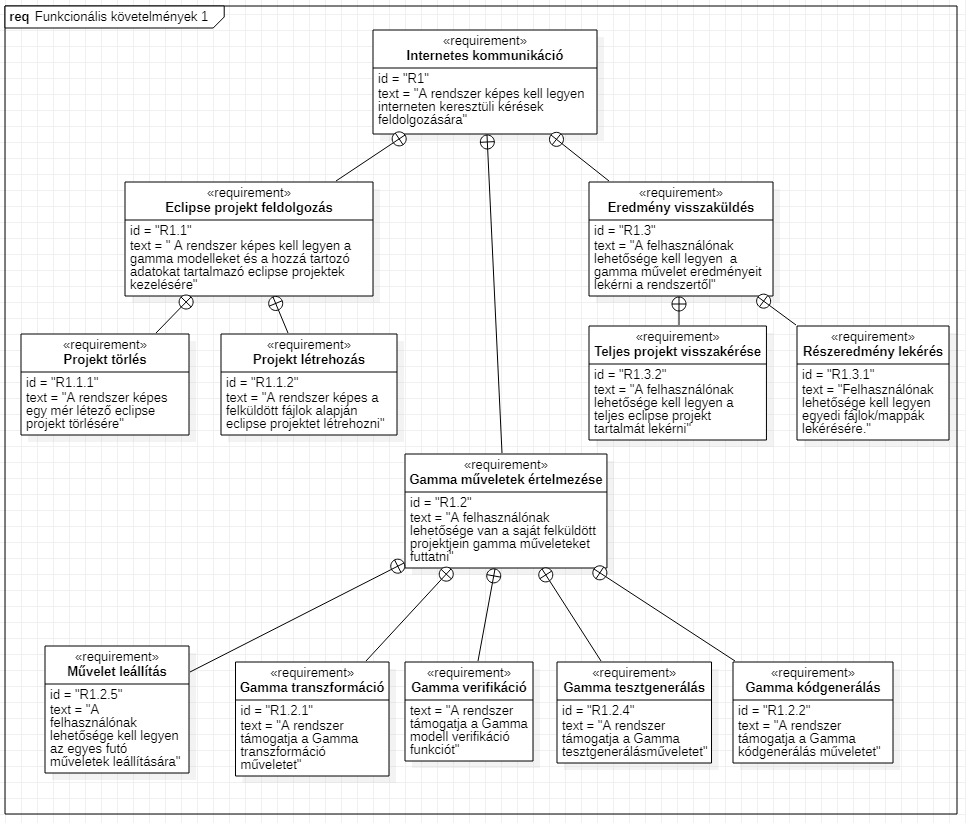
\includegraphics[width=170mm, keepaspectratio]{figures/requierments_placeholder.png}
	\caption{Követelmény hierarchia 1}
	\label{fig:requierments_placeholder}
\end{figure}

\begin{figure}[!ht]
	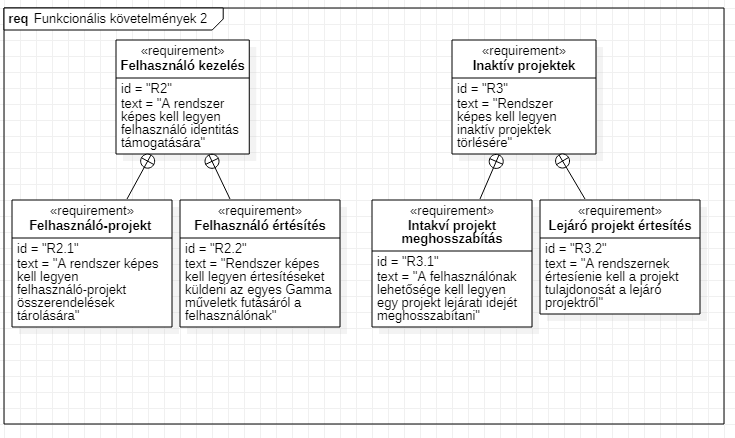
\includegraphics[width=150mm, keepaspectratio]{figures/requierments_2.png}
	\caption{Követelmény hierarchia 2}
	\label{fig:requierements_2}
\end{figure}

További nem funkcionális követelményeket négy kategóriába soroljuk:
\begin{itemize}
	\item \textbf{Megbízhatóság:} Egy projekten nem futtathatunk két különböző Gamma művelet halmazt
	\item \textbf{Biztonság:} Minden felhasználó csak a saját projektjeit szerkesztheti / saját projektjein futtathat gamma művelet halmazokat / A rendszer képes kell legyen kiszűrni az egyes rosszindulatú felhasználók által megadott fájl elérési utakat / 
	\item \textbf{Teljesítmény:} A rendszer képes kell legyen különböző projekteken ugyanabban az időben Gamma műveletek futtatására. / A rendszer skálázható kell legyen. / A rendszernek nem szabad fölösleges adatot tárolnia. / A rendszer muszáj töröljön minden olyan adatot, amely neki vagy a felhasználó számára nem releváns. / A rendszer képes kell legyen asszinkron módban működni.
	\item \textbf{Felhasználhatóság:} A rendszer megfelelő, HTTP szabvány által előírt válaszokat adni az egyes kérésekre. / A rendszer beszédes értesítéseket kell küldjön a projekt tulajdonosának az egyes Gamma műveletek futási állapotáról.
\end{itemize}

A fentebb leírt egyes követelmények bizonyos iniciális technológiai irány választásokat 

